\setcounter{section}{2}
\section{ĐƯỜNG TIỆM CẬN CỦA ĐỒ THỊ HÀM SỐ}
\subsection{LÝ THUYẾT CẦN NHỚ}
\subsubsection{Đường tiệm cận ngang (TCN):}
\begin{enumerate}[\iconMT]
	\item \indam{Định nghĩa:} Đường thẳng $y=m$ được gọi là một \inden{đường tiệm cận ngang} (hay \inden{tiệm cận ngang}) của đồ thị hàm số $y=f(x)$ nếu 
	$$\lim\limits_{x \rightarrow-\infty} f(x)=m \text{ hoặc }\lim\limits_{x \rightarrow+\infty} f(x)=m.$$
Đường thẳng $y=m$ là tiệm cận ngang của đồ thị hàm số $y=f(x)$ được minh hoạ như hình bên dưới\\
	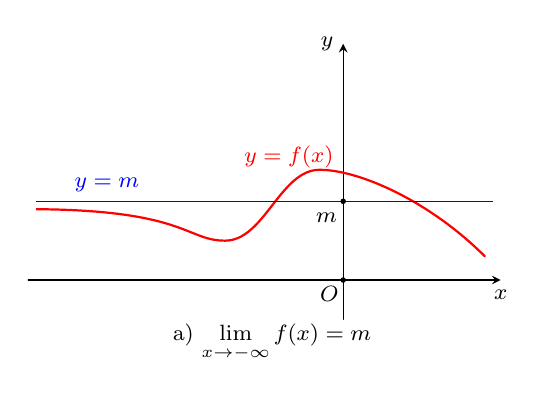
\begin{tikzpicture}[scale=1,>=stealth, font=\footnotesize, line join=round, line cap=round]
		\def\xmin{-4} \def\xmax{2}
		\def\ymin{-0.5} \def\ymax{3}
		%\draw[color=gray!50,dashed] (\xmin,\ymin) grid (\xmax,\ymax);
		\draw[->] (\xmin,0)--(\xmax,0) node [below]{$x$};
		\draw[->] (0,\ymin)--(0,\ymax) node [left]{$y$};
		\fill (0,0) circle (1pt) node[shift={(-135:2.5mm)}]{$O$};
		\node at (current bounding box.south) [below=-2pt] {a) $\lim\limits_{x \rightarrow-\infty} f(x)=m$};
		\clip (\xmin+0.1,\ymin+0.1) rectangle (\xmax-0.1,\ymax-0.1);
		\draw[red,thick,smooth,samples=300,domain=\xmin:\xmax]
		(-4,0.9)..controls +(0:2) and +(180:0.5)
		..(-1.5,0.5)..controls +(0:0.5) and +(180:0.5)
		..(-0.3,1.4)..controls +(0:0.5) and +(135:1)
		..(1.8,0.3);
		\draw [blue](\xmin,1)--(\xmax,1);
		\path[blue] (-3,1)node[above]{$y=m$};
		\path[red] (0,1.3)node[above left]{$y=f(x)$};
		\fill (0,1) circle (1pt) node[shift={(-135:3mm)}]{$m$};
	\end{tikzpicture}\hspace*{.5cm}
	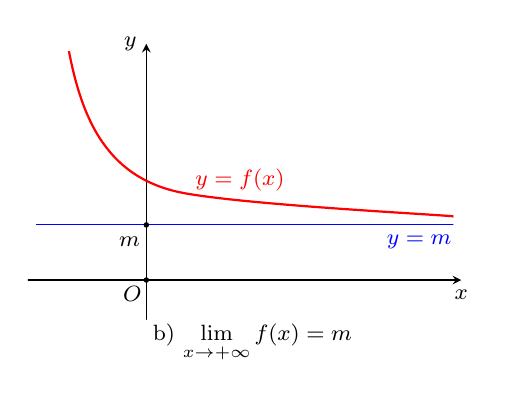
\begin{tikzpicture}[scale=1,>=stealth, font=\footnotesize, line join=round, line cap=round]
		\def\xmin{-1.5} \def\xmax{4}
		\def\ymin{-0.5} \def\ymax{3}
		%\draw[color=gray!50,dashed] (\xmin,\ymin) grid (\xmax,\ymax);
		\draw[->] (\xmin,0)--(\xmax,0) node [below]{$x$};
		\draw[->] (0,\ymin)--(0,\ymax) node [left]{$y$};
		\fill (0,0) circle (1pt) node[shift={(-135:2.5mm)}]{$O$};
		\node at (current bounding box.south) [below=-2pt] {b) $\lim\limits_{x \rightarrow+\infty} f(x)=m$};
		\clip (\xmin+0.1,\ymin+0.1) rectangle (\xmax-0.1,\ymax-0.1);
		\draw[red,thick,smooth,samples=300,domain=\xmin:\xmax]
		(-1,3)..controls +(-80:1) and +(170:1)
		..(0.5,1.1)..controls +(170:-1) and +(180:-0.5)
		..(3.9,0.8);
		\draw [blue](\xmin,0.7)--(\xmax,0.7);
		\path[blue] (4,0.7)node[below left]{$y=m$};
		\path[red] (0.5,1)node[above right]{$y=f(x)$};
		\fill (0,0.7) circle (1pt) node[shift={(-135:3mm)}]{$m$};
	\end{tikzpicture}
	\item \indam{Các bước tìm TCN:}
	\begin{boxdn}
		\begin{listEX}[1]
			\item [\ding{172}] Tính $\lim \limits_{x \to +\infty} f(x)$ và $\lim \limits_{x \to -\infty} f(x)$.
			\item [\ding{173}] Xem ở "vị trí" nào ra kết quả hữu hạn thì ta kết luận có tiệm cận ngang ở "vị trí" đó.
		\end{listEX}
	\end{boxdn}
\end{enumerate}
\subsubsection{Đường tiệm cận đứng (TCĐ)}
\begin{enumerate}[\iconMT]
	\item \indam{Định nghĩa:}	Đường thẳng $x=a$ được gọi là một \inden{đường tiệm cận đứng} (hay \inden{tiệm cận đứng}) của đồ thị hàm số $y=f(x)$ nếu ít nhất một trong các điều kiện sau thoả mãn:		
	$$
	\lim\limits_{x \rightarrow a^{-}} f(x)=+\infty,\,\, \lim\limits_{x \rightarrow a^{+}} f(x)=+\infty,\,\, \lim\limits_{x \rightarrow a^{-}} f(x)=-\infty,\,\, \lim\limits_{x \rightarrow a^{+}} f(x)=-\infty \text {. }
	$$
		Đường thẳng $x=a$ là tiệm cận đứng của đồ thị hàm số $y=f(x)$ được minh hoạ như hình bên dưới.\\
		\begin{center}
		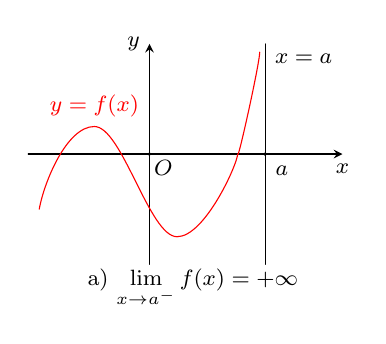
\begin{tikzpicture}[scale=.7,>=stealth, font=\footnotesize, line join=round, line cap=round]
			%Hình a
			\def\xmin{-2.2} \def\xmax{3.5}
			\def\ymin{-2} \def\ymax{2} 
			%\draw[color=gray!50,dashed] (\xmin,\ymin) grid (\xmax,\ymax); 
			\draw[->] (\xmin,0)--(\xmax,0) node [below]{$x$};
			\draw[->] (0,\ymin)--(0,\ymax) node [left]{$y$};
			\fill (0,0) circle (1pt) node[shift={(-45:2.5mm)}]{$O$};
			\draw (2.1,\ymin)--(2.1,\ymax)node[below right]{$x=a$};
			\fill (2.1,0) circle (1pt) node[shift={(-45:3mm)}]{$a$};
			%\clip (\xmin+0.1,\ymin+0.1) rectangle (\xmax-0.1,\ymax-0.1);
			\draw[red] (-2,-1)..controls +(80:0.5) and +(0:-.5)..(-1,0.5)node[above]{$y=f(x)$}
			..controls +(0:0.5) and +(180:0.5)..(0.5,-1.5)
			..controls +(0:0.5) and +(87:-0.2)..(1.6,0)
			..controls +(87:-.2) and +(90:-0.2)
			..(2,1.85);
			\node at (current bounding box.south) [below=-2pt] {a) $\lim\limits_{x \rightarrow a^{-}} f(x)=+\infty$};
		\end{tikzpicture}
		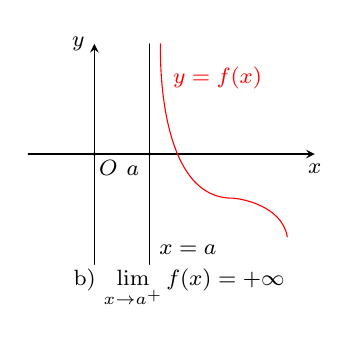
\begin{tikzpicture}[scale=.7,>=stealth, font=\footnotesize, line join=round, line cap=round]
			%Hình b
			\def\xmin{-1.2} \def\xmax{4}
			\def\ymin{-2} \def\ymax{2} 
			%\draw[color=gray!50,dashed] (\xmin,\ymin) grid (\xmax,\ymax); 
			\draw[->] (\xmin,0)--(\xmax,0) node [below]{$x$};
			\draw[->] (0,\ymin)--(0,\ymax) node [left]{$y$};
			\fill (0,0) circle (1pt) node[shift={(-45:2.5mm)}]{$O$};
			\draw (1,\ymin)node[above right]{$x=a$}--(1,\ymax);
			\fill (1,0) circle (1pt) node[shift={(-135:3mm)}]{$a$};
			\path[red] (1.25,1)node[above right]{$y=f(x)$};
			%\clip (\xmin+0.1,\ymin+0.1) rectangle (\xmax-0.1,\ymax-0.1);
			\draw[red] (1.2,2)..controls +(80:0) and +(0:-1.4)..(2.5,-0.8)
			..controls +(0:0.1) and +(-80:-0.6)
			..(3.5,-1.5);
			\node at (current bounding box.south) [below=-2pt] {b) $\lim\limits_{x \rightarrow a^{+}} f(x)=+\infty$};		
		\end{tikzpicture}\\
		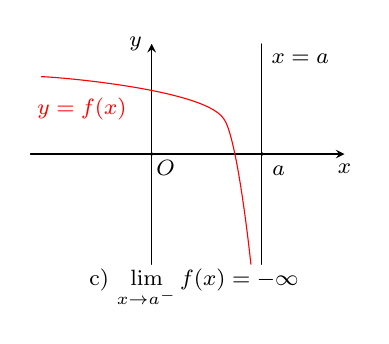
\begin{tikzpicture}[scale=.7,>=stealth, font=\footnotesize, line join=round, line cap=round]
			%Hình c
			\def\xmin{-2.2} \def\xmax{3.5}
			\def\ymin{-2} \def\ymax{2} 
			%\draw[color=gray!50,dashed] (\xmin,\ymin) grid (\xmax,\ymax); 
			\draw[->] (\xmin,0)--(\xmax,0) node [below]{$x$};
			\draw[->] (0,\ymin)--(0,\ymax) node [left]{$y$};
			\fill (0,0) circle (1pt) node[shift={(-45:2.5mm)}]{$O$};
			\draw (2,\ymin)--(2,\ymax)node[below right]{$x=a$};
			\fill (2,0) circle (1pt) node[shift={(-45:3mm)}]{$a$};
			\path[red] (-2.25,1.2)node[below right]{$y=f(x)$};
			%\clip (\xmin+0.1,\ymin+0.1) rectangle (\xmax-0.1,\ymax-0.1);
			\draw[red] (-2,1.4)..controls +(-10:-0.2) and +(-55:-.7)
			..(1.3,0.65)..controls +(-50:0.4) and +(-90:0)
			..(1.8,-2)
			;
			\node at (current bounding box.south) [below=-2pt] {c) $\lim\limits_{x \rightarrow a^{-}} f(x)=-\infty$};		
		\end{tikzpicture}
		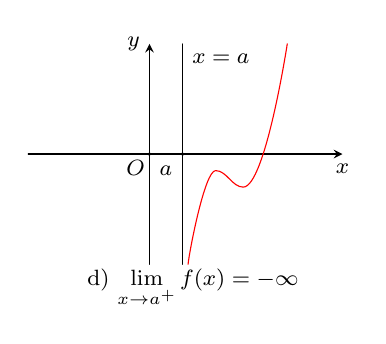
\begin{tikzpicture}[scale=.7,>=stealth, font=\footnotesize, line join=round, line cap=round]
			%Hình d
			\def\xmin{-2.2} \def\xmax{3.5}
			\def\ymin{-2} \def\ymax{2} 
			%\draw[color=gray!50,dashed] (\xmin,\ymin) grid (\xmax,\ymax); 
			\draw[->] (\xmin,0)--(\xmax,0) node [below]{$x$};
			\draw[->] (0,\ymin)--(0,\ymax) node [left]{$y$};
			\fill (0,0) circle (1pt) node[shift={(-135:2.5mm)}]{$O$};
			\draw (.6,\ymin)--(.6,\ymax)node[below right]{$x=a$};
			\fill (.6,0) circle (1pt) node[shift={(-135:3mm)}]{$a$};
			%\clip (\xmin+0.1,\ymin+0.1) rectangle (\xmax-0.1,\ymax-0.1);
			\draw[red] (0.7,-2)..controls +(85:0.2) and +(180:0.2)
			..(1.2,-0.3)..controls +(0:0.2) and +(180:0.2)
			..(1.7,-0.6)..controls +(0:0.4) and +(90:0)
			..(2.5,2)
			;
			\node at (current bounding box.south) [below=-2pt] {d) $\lim\limits_{x \rightarrow a^{+}} f(x)=-\infty$};		
		\end{tikzpicture}
	\end{center}
	\item \indam{Các bước tìm TCĐ:}
	\begin{boxdn}
		\begin{listEX}[1]
			\item [\ding{172}] Tìm nghiệm của mẫu, giả sử nghiệm đó là $x=x_0$.
			\item [\ding{173}] Tính giới hạn một bên tại $x_0$. Nếu xảy ra $\lim \limits_{x \to x_0^{-}} f(x) =\infty \text{ hoặc} \lim \limits_{x \to x_0^{+}} f(x) =\infty$
			thì ta kết luận $x=x_0$ là đường tiệm cận đứng.
		\end{listEX}
	\end{boxdn}
\end{enumerate}
\subsubsection{Đường tiệm cận xiên}
\begin{enumerate}[\iconMT]
	\item \indam{Định nghĩa:} Đường thẳng $y=ax+b$, $a \neq 0$, được gọi là \inden{đường tiệm cận xiên} (hay \inden{tiệm cận xiên}) của đồ thị hàm số $y=f(x)$ nếu 
	$$\lim\limits_{x \rightarrow-\infty}[f(x)-(ax+b)]=0 \text{ hoặc }\lim\limits_{x \rightarrow+\infty}[f(x)-(ax+b)]=0.$$
	Đường thẳng $y=ax+b$ là tiệm cận xiên của đồ thị hàm số $y=f(x)$ được minh hoạ như hình bên dưới:\\	
		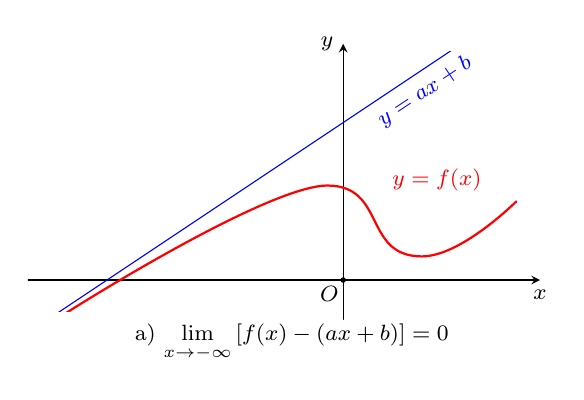
\begin{tikzpicture}[scale=1,>=stealth, font=\footnotesize, line join=round, line cap=round]
			\def\xmin{-4} \def\xmax{2.5}
			\def\ymin{-0.5} \def\ymax{3}
			%\draw[color=gray!50,dashed] (\xmin,\ymin) grid (\xmax,\ymax);
			\draw[->] (\xmin,0)--(\xmax,0) node [below]{$x$};
			\draw[->] (0,\ymin)--(0,\ymax) node [left]{$y$};
			\fill (0,0) circle (1pt) node[shift={(-135:2.5mm)}]{$O$};
			\node at (current bounding box.south) [below=-2pt] {a) $\lim\limits_{x \rightarrow-\infty}\left[f(x)-(ax+b)\right]=0$};
			\clip (\xmin+0.1,\ymin+0.1) rectangle (\xmax-0.1,\ymax-0.1);
			\draw[red,thick,smooth,samples=300,domain=\xmin:\xmax]
			(-3.8,-0.6)..controls +(34:0.5) and +(180:.75)
			..(-0.2,1.2)..controls +(0:0.75) and +(180:.75)
			..(1,0.3)..controls +(0:0.5) and +(80:0)
			..(2.2,1);
			\draw[blue,smooth,samples=300,domain=\xmin:\xmax] plot(\x,{2/3*(\x)+2});
			\path[blue] (-3,0)--(0,2)node[below,sloped,pos=1.3]{$y=ax+b$};
			\path[red] (0.5,1)node[above right]{$y=f(x)$};
		\end{tikzpicture}\hspace{.5cm}
		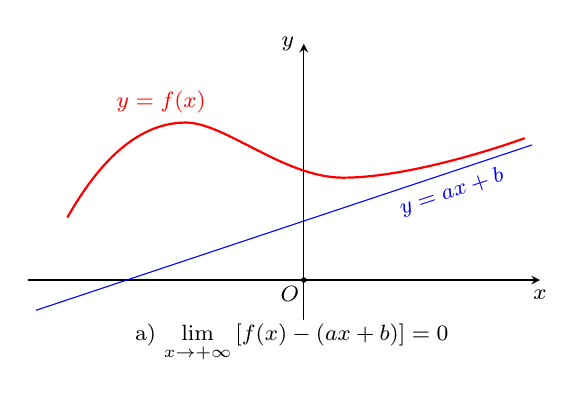
\begin{tikzpicture}[scale=1,>=stealth, font=\footnotesize, line join=round, line cap=round]
			\def\xmin{-3.5} \def\xmax{3}
			\def\ymin{-0.5} \def\ymax{3}
			%\draw[color=gray!50,dashed] (\xmin,\ymin) grid (\xmax,\ymax);
			\draw[->] (\xmin,0)--(\xmax,0) node [below]{$x$};
			\draw[->] (0,\ymin)--(0,\ymax) node [left]{$y$};
			\fill (0,0) circle (1pt) node[shift={(-135:2.5mm)}]{$O$};
			\node at (current bounding box.south) [below=-2pt] {a) $\lim\limits_{x \rightarrow+\infty}\left[f(x)-(ax+b)\right]=0$};
			\clip (\xmin+0.1,\ymin+0.1) rectangle (\xmax-0.1,\ymax-0.1);
			\draw[red,thick,smooth,samples=300,domain=\xmin:\xmax]
			(-3,0.8)..controls +(60:0.5) and +(180:.75)
			..(-1.5,2)..controls +(0:.5) and +(180:.75)
			..(0.5,1.3)..controls +(0:.75) and +(-160:.5)
			..(2.8,1.8);
			\draw[blue,smooth,samples=300,domain=\xmin:\xmax] plot(\x,{1/3*(\x)+0.75});
			\path[blue] (-3,-0.25)--(0,0.75)node[below,sloped,pos=1.6]{$y=ax+b$};
			\path[red] (-2.5,2)node[above right]{$y=f(x)$};
		\end{tikzpicture}
	\item \indam{Các bước tìm TCX y = ax + b:}
	Ta xác định hệ số của $a$ và $b$ trong 2 trường hợp sau:
	\begin{boxdn}
		\begin{listEX}[1]
			\item [\ding{172}] Tính $a=\lim\limits_{x \rightarrow+\infty} \dfrac{f(x)}{x}$, $b=\lim\limits_{x \rightarrow+\infty}[f(x)-ax]$.
			\item [\ding{173}] Tính $a=\lim\limits_{x \rightarrow-\infty} \dfrac{f(x)}{x}$, $b=\lim\limits_{x \rightarrow-\infty}[f(x)-ax]$.
		\end{listEX}
	\end{boxdn}
\end{enumerate}
\subsection{PHÂN LOẠI VÀ PHƯƠNG PHÁP GIẢI TOÁN}
\begin{dang}{Bài toán tìm tiệm cận đứng và tiệm cận ngang của đồ thị hàm số}
	Cho hàm số $y=f(x)$. Để tìm tiệm cận đứng và tiệm cận ngang, ta làm như sau:
	\begin{enumerate}[\iconCH]
		\item \indamm{Các bước tìm tiệm cận đứng:}
		\begin{listEX}[1]
			\item [\ding{172}] Tìm nghiệm của mẫu, giả sử nghiệm đó là $x=x_0$.
			\item [\ding{173}] Tính giới hạn một bên tại $x_0$. Nếu xảy ra $\lim \limits_{x \to x_0^{-}} f(x) =\infty \text{ hoặc} \lim \limits_{x \to x_0^{+}} f(x) =\infty$
			thì ta kết luận $x=x_0$ là đường tiệm cận đứng.
		\end{listEX}
		\item \indamm{Các bước tìm tiệm cận ngang:}
		\begin{listEX}[1]
			\item [\ding{172}] Tính $\lim \limits_{x \to +\infty} f(x)$ và $\lim \limits_{x \to -\infty} f(x)$.
			\item [\ding{173}] Xem ở "vị trí" nào ra kết quả hữu hạn thì ta kết luận có tiệm cận ngang ở "vị trí" đó.
		\end{listEX}
		\item \indamm{Lưu ý:} Đồ thị hàm số $y=\dfrac{ax+b}{cx+d}$ luôn có TCĐ $x=-\dfrac{d}{c}$ và TCN: $y=\dfrac{a}{c}$.
	\end{enumerate}
\end{dang}
\boxmini{BÀI TẬP TỰ LUẬN}
\begin{vd}
	Xác định tiệm cận đứng và tiệm cận ngang của đồ thị hàm số cho bởi công thức sau:
	\begin{enumEX}[a)]{4}
		\item $y=\dfrac{2x-1}{x+1}$;
		\item $y=\dfrac{2 x-3}{1-2 x}$;
		\item $y=\dfrac{x^2-5x+4}{x^2-1}$;
		\item $y=\dfrac{2x-1}{x^2-3x+2}$.
	\end{enumEX}
\loigiai{
\begin{enumerate}[a)]
	\item Xét $\lim\limits_{x \to -1^+} \dfrac{2x-1}{x+1}=-\infty$ (hoặc $\lim\limits_{x \to -1^-} \dfrac{2x-1}{x+1}=+\infty$) nên đường thẳng $x=-1$ là tiệm cận đứng.\\
	Xét $\lim\limits_{x \to \pm \infty } \dfrac{2x-1}{x+1}=2$ nên đường thẳng $y=2$ là tiệm cận ngang.
	\item Ta có
	\begin{itemize}
		\item $\lim\limits_{x \to \pm\infty} y=\lim\limits_{x \to \pm\infty} \dfrac{2x-3}{1-2x}=-1$ suy ra $y=-1$ là tiệm cận ngang.
		\item $\heva{& \lim\limits_{x \to \tfrac{1}{2}^+} \dfrac{2x-3}{1-2x}=+\infty \\ & \lim\limits_{x \to \tfrac{1}{2}^-} \dfrac{2x-3}{1-2x}=-\infty}$ suy ra $x=\dfrac{1}{2}$ là tiệm cận đứng.
	\end{itemize}
	\item Điều kiện xác định: $\heva{&x\neq-1\\ &x\neq1.}$
	\begin{itemize}
		\item $\lim\limits_{x\to\pm\infty}\dfrac{x^2-5x+4}{x^2-1}=1$
		\item $\lim\limits_{x\to(-1)^-}\dfrac{x^2-5x+4}{x^2-1}=+\infty$
		\item $\lim\limits_{x\to1}\dfrac{x^2-5x+4}{x^2-1}=-\dfrac{3}{2}$
	\end{itemize}
	Vậy đồ thị hàm số có một tiệm cận ngang $y=1$ và một tiệm cận đứng $x=-1$.
	\item Tập xác định $\mathscr{D}=\mathbb{R}\setminus\{1; 2\}$.\\
	Ta có\begin{itemize}
		\item $\lim\limits_{x\to\pm\infty}y=\lim\limits_{x\to\pm\infty}\dfrac{2x-1}{x^2-3x+2}=0$ nên $y=0$ là đường tiệm cận ngang.
		\item $\lim\limits_{x\to 1^-}y=\lim\limits_{x\to 1^-}\dfrac{2x-1}{x^2-3x+2}=\lim\limits_{x\to 1^-}\dfrac{2x-1}{(x-1)(x-2)}=+\infty$ và $\lim\limits_{x\to 1^+}y=-\infty$ nên $x=1$ là đường tiệm cận đứng.
		\item $\lim\limits_{x\to 2^-}y=\lim\limits_{x\to 2^-}\dfrac{2x-1}{x^2-3x+2}=\lim\limits_{x\to 2^-}\dfrac{2x-1}{(x-1)(x-2)}=-\infty$ và $\lim\limits_{x\to 2^+}y=2=+\infty$ nên $x=2$ là đường tiệm cận đứng.
	\end{itemize}
\end{enumerate}}
\end{vd}

\boxmini{BÀI TẬP TRẮC NGHIỆM}
\ind{PHẦN I.} \inden{Câu trắc nghiệm nhiều phương án lựa chọn. Mỗi câu hỏi học sinh chỉ chọn một phương án.}\\
\setcounter{ex}{0}
\Opensolutionfile{ans}[ans/2D1-B3-d1-1]
\begin{ex}
	Đường tiệm cận ngang của đồ thị hàm số $y=\dfrac{2x-4}{x+2}$ là
	\choice
	{\True $y=2$}
	{  $x=2$}
	{ $x=-2$}
	{$y=-2$}
	
	\loigiai{$\underset{x\to -\infty }{\mathop{\lim \limits_{n \to +\infty}}}\,\dfrac{2x-4}{x+2}=2$ và $\underset{x\to +\infty }{\mathop{\lim \limits_{n \to +\infty}}}\,\dfrac{2x-4}{x+2}=2$ nên hàm số có tiệm cận ngang là $y=2$.
	}
\end{ex}

\begin{ex}
	Tìm tiệm cận ngang của đồ thị hàm số $ y = \dfrac{2x + 1}{ x +1} $.
	\choice
	{ \True $  y = -2 $}
	{$  x = -2 $}
	{ $  y = 2 $}
	{$ x = 1 $}
	\loigiai{
		Ta có $ \displaystyle \lim_{ x \rightarrow \pm \infty } \dfrac{2x + 1}{-x + 1} = -2  $.	
	}		
\end{ex}

\begin{ex}
	Đường thẳng $y=3$ là tiệm cận ngang của đồ thị hàm số nào sau đây?
	\choice
	{$y=\dfrac{1-3x}{2+x}$}
	{$y=\dfrac{x^2+3x+2}{x-2}$}
	{\True $y=\dfrac{1+3x}{1+x}$}
	{$y=\dfrac{3x^2+2}{2-x}$}
	\loigiai{
		Ta có $\lim\limits_{x\to \pm \infty}\dfrac{1+3x}{1+x}=3$ nên $y=3$ là tiệm cận ngang của đồ thị hàm số $y=\dfrac{1+3x}{1+x}$.}
\end{ex}

\begin{ex}
	Hàm số nào có đồ thị nhận đường thẳng $x = 2$ làm đường tiệm cận đứng?
	\choice
	{$y=x-2+\dfrac{1}{x+1}$}
	{$y=\dfrac{1}{x+1}$}
	{$y=\dfrac{2}{x+2}$}
	{\True $y=\dfrac{5x}{2-x}$}
	\loigiai{ Xét hàm số $y=\dfrac{5x}{2-x}$\\
		Ta có $\lim\limits_{x\to 2^+}5x=10>0$; $\lim\limits_{x\to 2^+}(2-x)$ và $x-2<0$ khi $x>2$ suy ra $\lim\limits_{x\to 2^+}\dfrac{5x}{2-x}=-\infty$.\\
		Vậy đồ thị hàm số $y=\dfrac{5x}{2-x}$ nhận đường thẳng $x=2$ làm tiệm cận đứng.
	}
\end{ex}

\begin{ex}
	Đường tiệm cận đứng của đồ thị hàm số $y=\dfrac{3x+1}{x-2}$ là đường thẳng
	\choice
	{$x=-2$}
	{\True $x=2$}
	{$y=3$}
	{$y=-\dfrac{1}{2}$}
	\loigiai{Ta có: $\lim \limits_{x\to 2^+}{\dfrac{3x+1}{x-2}}=+\infty$.
	}
\end{ex}

\begin{ex}
	Đường tiệm cận đứng của đồ thị hàm số $y=\dfrac{x+1}{x^2+4x-5}$ có phương trình là
	\choice
	{$x=-1$}
	{$y=1;y=-5$}
	{\True $x=1;x=-5$}
	{$x=\pm 5$}
	\loigiai{
		Ta có $\mathop{\lim}\limits_{x\rightarrow 1^+}y=+\infty$, $\mathop{\lim}\limits_{x\rightarrow 1^-}y=-\infty$, $\mathop{\lim}\limits_{x\rightarrow 5^+}y=+\infty$, $\mathop{\lim}\limits_{x\rightarrow 5^-}y=-\infty$.\\
		Vậy đồ thị hàm số có hai đường tiệm cận đứng là $x=1$ và $x=-5$.}
\end{ex}

\begin{ex}
	Tìm số đường tiệm cận của đồ thị hàm số $ y = \dfrac{x^2 - 3x + 2}{x^2 - 4}. $
	\choice
	{$1$}
	{$ 0$}
	{\True $2$}
	{$3$}
	\loigiai
	{
		Tập xác định: $ \mathscr D = \mathbb{R} \backslash \{\pm2 \} $.\\
		Ta có $ \lim \limits_{x \to \pm  \infty} y = 1 \Rightarrow  $ đồ thị hàm số có 1 tiệm cận ngang là $ y = 1. $\\
		Ta lại có $\lim \limits_{x \to 2} y =  \lim \limits_{x \to 2} \dfrac{x-1}{x+2} = \dfrac{1}{4} $ và $\lim \limits_{x \to -2^+} y =  \lim \limits_{x \to -2^+} \dfrac{x-1}{x+2} = -\infty$ nên đồ thị hàm số có 1 tiệm cận đứng là $ x = -2. $\\
		Vậy đồ thị hàm số đã cho có 2 đường tiệm cận.
	}
\end{ex}

\begin{ex}
	Số đường tiệm cận của đồ thị hàm số $y=\dfrac{3}{x-2}$ là
	\choice
	{$1$}
	{\True $2$}
	{$0$}
	{$3$}
	\loigiai{
		Tiệm cận đứng $x=2$.\\
		Tiệm cận ngang $y=0$.
	}
\end{ex}

\begin{ex}
	Cho hàm số $y=f(x)$ có đồ thị là đường cong $(C)$ và các giới hạn $\lim\limits_{x\to 2^{+}}f(x)=1$, $\lim\limits_{x\to 2^{-}}f(x)=1$, $\lim\limits_{x\to +\infty}f(x)=2$, $\lim\limits_{x\to -\infty}f(x)=2$. Hỏi mệnh đề nào sau đây đúng?
	\choice
	{\True Đường thẳng $y=2$ là tiệm cận ngang của $(C)$}
	{Đường thẳng $y=1$ là tiệm cận ngang của $(C)$}
	{Đường thẳng $x=2$ là tiệm cận ngang của $(C)$}
	{Đường thẳng $x=2$ là tiệm cận đứng của $(C)$}
	\loigiai{
		Ta có $\lim\limits_{x\to +\infty}f(x)=2$, $\lim\limits_{x\to -\infty}f(x)=2\Rightarrow y=2$ là tiệm cận ngang của $(C)$.
	}
\end{ex}

\begin{ex}
	Số tiệm cận đứng của đồ thị hàm số $y=\dfrac{\sqrt{x+9}-3}{x^2+x}$ là
	\choice
	{$3$}
	{$2$}
	{$0$}
	{\True $1$}
	\loigiai{
		Tập xác định $\mathscr{D}=[-9;+\infty)\setminus \{-1;0\}$. \\
		Ta có $\left\{\begin{aligned}
			&\lim\limits_{x\to -1^+} \dfrac{\sqrt{x+9}-3}{x^2+x}=+\infty \\
			&\lim\limits_{x\to -1^-} \dfrac{\sqrt{x+9}-3}{x^2+x}=-\infty
		\end{aligned}\right. \Rightarrow x=-1$ là tiệm cận đứng. \\
		Ngoài ra $\lim\limits_{x\to 0} \dfrac{\sqrt{x+9}-3}{x^2+x}=\dfrac{1}{6}$ nên $x=0$ không thể là một tiệm cận được.}
\end{ex} 

\begin{ex}%[2D1B4]
	\immini{Cho hàm số $y=f(x)$ xác định trên $\mathbb{R}\setminus\left\{\pm1\right\}$ liên tục trên mỗi khoảng xác định và có bảng biến thiên như hình vẽ. Số đường tiệm cận của đồ thị hàm số là
	\choice
	{$1$}
	{$2$}
	{\True $3$}
	{$4$}}{\hspace{0.5cm}

\begin{tikzpicture}
	\tikzset{double style/.append style = {draw=\tkzTabDefaultWritingColor,double=\tkzTabDefaultBackgroundColor,double distance=2pt}}
	\tikzset{double style/.append style = {double distance=0.5pt}} 
	\tkzTabInit[nocadre=false,lgt=1,espcl=1.7]
	{$x$/.7,$y'$ /.7, $y$ /2.3}
	{$-\infty$ ,$-1$,$0$,$1$,$+\infty$}
	\tkzTabLine{,-,d,-,0,+,d,+,}
	\tkzTabVar {+/$-2$,-D+/$-\infty$/$+\infty$,-/$1$,+D-/$+\infty$/$-\infty$,+/$-2$}
\end{tikzpicture}}
	\loigiai{
		Dựa vào bảng biến thiên ta có:\\
		$\lim\limits_{x\to -1^\pm}f(x)=\pm\infty$. 
		$\lim\limits_{x\to 1^\pm}f(x)=\mp\infty$.\\
		Do đó $x=1$ và $x=-1$ là các đường tiệm cận đứng của đồ thị hàm số.\\
		Lại có $\lim\limits_{x\to \pm\infty}f(x)=-2$. Do đó $y=-2$ là tiệm cận ngang của đồ thị hàm số.\\
		Vậy đồ thị hàm số có $3$ đường tiệm cận.
	}
\end{ex}

\begin{ex}
	\immini{Cho hàm số $y=f(x)$ xác định trên $\mathbb{R}\backslash \left\{0\right\},$ liên tục trên mỗi khoảng xác định và có bảng biến thiên như hình bên. Chọn khẳng định đúng.
	\choice
	{Đồ thị hàm số có đúng một tiệm cận ngang}
	{Đồ thị hàm số có hai tiệm cận ngang}
	{\True Đồ thị hàm số có đúng một tiệm cận đứng}
	{Đồ thị hàm số không có tiệm đứng và tiệm cận ngang}}{
	
\begin{tikzpicture}[>=stealth]
		\tikzset{double style/.append style = {draw=\tkzTabDefaultWritingColor,double=\tkzTabDefaultBackgroundColor,double distance=2pt}}
		\tkzTabInit[nocadre=false,lgt=1,espcl=2]{$x$/.6,$y'$/.7,$y$/2}{$-\infty$,$0$,$1$,$+\infty$}
		\tkzTabLine{,-, d ,+,z,-,} 
		\tkzTabVar{+/$+\infty$ / , -D- / $-1$ /$-\infty$,+/$2$,-/$-\infty$}
\end{tikzpicture}}
	\loigiai{
		Do $\lim\limits_{x \to +\infty} y=-\infty$ và $\lim\limits_{x \to -\infty} y=+\infty$  nên đồ thị hàm số không có tiệm cận ngang.\\
		Do $\lim\limits_{x \to 0^+} y=+\infty$ suy ra $x=0$ là tiệm cận đứng của đồ thị hàm số.
	} 
\end{ex}

\begin{ex}
	\immini{Cho hàm số $ y=f(x) $ có bảng biến thiên như hình bên. Hỏi đồ thị hàm số đã cho có bao nhiêu đường tiệm cận?
	\choice
	{\True $ 2 $}
	{$ 3 $}
	{$ 4 $}
	{$ 1 $}}{
\begin{tikzpicture}[yscale=.8,xscale=1.15,
	kxd/.pic={\draw[double] (90:.4)--(-90:.4);}]
	\begin{scope}[shift={(-.5,.5)}]
		\fill[pattern=north east lines,pattern color=black]
		(1,-1) rectangle +(1.45,-4);
		\draw
		(0,0) rectangle +(7,-5)
		(0,-1)--+(0:7) (0,-2)--+(0:7) (1,0)--+(-90:5);
	\end{scope}
	\path
	(0,0) node{$ x $}
	++ (0:1) node{$ -\infty $}
	++(0:1)node{$ -2 $}
	++(0:2)node{$ 0 $}
	++(0:2)node{$ +\infty $}
	(0,-1)node{$ y' $}
	++(0:2)pic{kxd}
	++(0:1)node{$ + $}
	++(0:1)pic{kxd}
	++(0:1)node{$ - $}
	(0,-3)node{$ y $}
	++(0:2)pic[yscale=3]{kxd}
	+(-90:1)node[below right](A){$ -\infty $}
	++(0:2) pic[yscale=3]{kxd}
	node[above right](C){$ 1 $}
	+(90:1)node[left](B){$ 2 $}
	++(0:2)node[below](D){$ 0 $};
	\draw[-stealth,black](A)--(B)
	;
	\draw[-stealth,black] (C)--(D);
\end{tikzpicture}}
	\loigiai{
		Dựa vào bảng biến thiên của hàm số, suy ra
		\begin{itemize}
			\item  $ \lim\limits_{x \to +\infty} f(x)=0 $, đồ thị hàm số có tiệm cận ngang là $ y=0 $.
			\item $ \lim\limits_{x \to (-2)^+} f(x)=-\infty $, đồ thị hàm số có tiệm cận đứng là $ x=-2 $.
			Vậy đồ thị hàm số đã cho có $ 2 $ đường tiệm cận.
		\end{itemize}
	}
\end{ex}

\Closesolutionfile{ans}

\ind{PHẦN II.} \inden{Câu trắc nghiệm đúng sai. Trong mỗi ý a), b), c), d) ở mỗi câu, học sinh chọn đúng hoặc sai.}\\
\Opensolutionfile{ans}[ans/2D1-B3-d1-2]
\begin{ex}
	Cho hàm số $y=f(x)$ có bảng biến thiên như hình bên. Xét tính đúng, sai của các khẳng định sau:
	\begin{center}
		
\begin{tikzpicture}
			\tikzset{double style/.append style = {draw=\tkzTabDefaultWritingColor,double=\tkzTabDefaultBackgroundColor,double distance=2pt}}
			\tkzTab[nocadre=false,lgt=1.2,espcl=1.7,deltacl=0.6]
			{$x$/0.6, $y'$/0.6, $y$/2}
			{$-\infty$, $0$, $2$, $+\infty$}
			{,-,d,-,$0$,+,}
			{+/ $2$, -D+/ $-\infty$ / $+\infty$, -/ $2$,+/$+\infty$}
		\end{tikzpicture}
	\end{center}
	\choiceTF
	{\True $f(-5)<f(4)$}
	{Hàm số có giá trị nhỏ nhất bằng $2$}
	{\True Đồ thị hàm số có tiệm cận đứng $x=0$}
	{Đồ thị hàm số không có tiệm cận ngang}
	\loigiai{
		\begin{enumerate}[a)]
			\item Từ bảng biến thiên ta thấy $f(-5)<2$ và $f(4)>2$ nên $f(-5)<f(4)$.
			\item Do $\lim \limits_{x\to 0^-}y=-\infty$ nên hàm số không có giá trị nhỏ nhất.
			\item Do $\lim \limits_{x\to 0^-}y=-\infty$ nên đồ thị hàm số có tiệm cận đứng $x=0$.
			\item Do $\lim \limits_{x\to -\infty}y=2y$ nên đồ thị hàm số có tiệm cận ngang $y=2$.
		\end{enumerate}
}
\end{ex}


\begin{ex}
	Cho hàm số hàm số $y=\dfrac{-4x+5}{2x+3}$ có đồ thị $(C)$.
	Xét tính đúng sai của các khẳng định sau:
	\choiceTF
	{\True Hàm số không có cực trị}
	{Đồ thị hàm số có tiệm cận đứng $x=-3$}
	{Đồ thị hàm số có tiệm cận ngang $y=-2$}
	{\True Các đường tiệm cận của đồ thị tạo với hai trục toạ độ một hình chữ nhật có diện tích bằng $3$}
	\loigiai{
		Tập xác định $\mathscr D=\mathbb{R}\setminus \left \{-\dfrac{3}{2}\right \}$\\
		$\lim \limits_{x\to \left (-\frac{3}{2}\right )^+}y=+\infty; \ \lim \limits_{x\to \left (-\frac{3}{2}\right )^-}y=-\infty$ nên đồ thị hàm số có tiệm cận đứng $x=-\dfrac{3}{2}$\\
		$\lim \limits_{x\to -\infty}y=-2, \ \lim \limits_{x\to +\infty}y=-2$ nên đồ thị hàm số có một tiệm cận ngang là $y=-2$\\
		Diện tích hình chữ nhật cần tìm là $S=\left |-\dfrac{3}{2}\right |\cdot \left |-2\right |=3$
	}
\end{ex}

\Closesolutionfile{ans}

\begin{dang}{Bài toán tìm tiệm cận đứng và tiệm cận xiên của đồ thị hàm số}
	\begin{enumerate}[\iconCH]
		\item \indamm{Các bước tìm TCX y = ax + b:}
		Ta xác định hệ số của $a$ và $b$ trong 2 trường hợp sau:
			\begin{listEX}[1]
				\item [\ding{172}] Tính $a=\lim\limits_{x \rightarrow+\infty} \dfrac{f(x)}{x}$, $b=\lim\limits_{x \rightarrow+\infty}[f(x)-ax]$.
				\item [\ding{173}] Tính $a=\lim\limits_{x \rightarrow-\infty} \dfrac{f(x)}{x}$, $b=\lim\limits_{x \rightarrow-\infty}[f(x)-ax]$.
			\end{listEX}
		\item \indamm{Lưu ý:} 
		\begin{listEX}[1]
			\item [\ding{172}] Nếu $a=0$ thì tiệm cận xiên chính là tiệm cận ngang.
			\item [\ding{173}] Đối với hàm số phân thức $f(x)=\dfrac{ax^2+bx+c}{mx+n}$, ta có thể chia đa thức, biến đổi về dạng
			$$f(x)=a'x+b'+\dfrac{e}{mx+n}, \, \text{ với } e \ne0$$
			Suy ra $y=a'x+b'$ là đường tiệm cận xiên của đồ thị hàm số.
		\end{listEX}
	\end{enumerate}
	
\end{dang}
\boxmini{BÀI TẬP TỰ LUẬN}

\begin{vd}
	Tìm các tiệm cận đứng và tiệm cận xiên của đồ thị hàm số sau:
	\begin{listEX}[3]
		\item $y=\dfrac{x^{2}+2}{2x-4}$;
		\item $y=\dfrac{2x^{2}-3x-6}{x+2}$;
		\item $y=\dfrac{2x^{2}+9x+11}{2x+5}$.
	\end{listEX}
	\loigiai{
		\begin{listEX}
			\item Hàm số $y=f(x)=\dfrac{x^{2}+2}{2x-4}$ có tập xác định $\mathscr{D}=\mathbb{R} \setminus \left\lbrace 2\right\rbrace$.
			\begin{itemize}
				\item Ta có $\lim\limits_{x \rightarrow 2^{-}} \dfrac{x^{2}+2}{2x-4}=-\infty$; $\lim\limits_{x \rightarrow 2^{+}} \dfrac{x^{2}+2}{2x-4}=+\infty$.\\
				Suy ra đường thẳng $x=2$ là một tiệm cận đứng của đồ thị hàm số.
				\item Ta có $\begin{aligned}[t]
					a&=\lim\limits_{x \rightarrow+\infty} \dfrac{f(x)}{x}=\lim\limits_{x \rightarrow+\infty} \dfrac{x+\dfrac{2}{x}}{2x-4}=\dfrac{1}{2};\\
					b&=\lim\limits_{x \rightarrow+\infty}[f(x)-ax]=\lim\limits_{x \rightarrow+\infty}\left(\dfrac{x^{2}+2}{2x-4}-\dfrac{1}{2}x\right)=\lim\limits_{x \rightarrow+\infty} \dfrac{2x+2}{2x-4}=1.
				\end{aligned}$\\
				Ta cũng có $\lim\limits_{x \rightarrow-\infty} \dfrac{f(x)}{x}=\dfrac{1}{2}$; $\lim\limits_{x \rightarrow-\infty}[f(x)-\dfrac{1}{2}x]=1$.
				\\
				Do đó, đồ thị hàm số có tiệm cận xiên là đường thẳng $y=\dfrac{1}{2}x+1$.
			\end{itemize}	
			\item Hàm số $y=f(x)=\dfrac{2x^{2}-3x-6}{x+2}$ có tập xác định $\mathscr{D}=\mathbb{R} \setminus \left\lbrace -2\right\rbrace$.
			\begin{itemize}
				\item Ta có $\lim\limits_{x \rightarrow \left(-2\right)^{-}} \dfrac{2x^{2}-3x-6}{x+2}=-\infty$; $\lim\limits_{x \rightarrow \left(-2\right)^{+}} \dfrac{2x^{2}-3x-6}{x+2}=+\infty$.\\
				Suy ra đường thẳng $x=-2$ là một tiệm cận đứng của đồ thị hàm số.
				\item Ta có $\begin{aligned}[t]
					a&=\lim\limits_{x \rightarrow+\infty} \dfrac{f(x)}{x}=\lim\limits_{x \rightarrow+\infty} \dfrac{2x-3-\dfrac{6}{x}}{x+2}=2;\\
					b&=\lim\limits_{x \rightarrow+\infty}[f(x)-ax]=\lim\limits_{x \rightarrow+\infty}\left(\dfrac{2x^{2}-3x-6}{x+2}-2x\right)=\lim\limits_{x \rightarrow+\infty} \dfrac{-7x-6}{x+2}=-7.
				\end{aligned}$\\
				Ta cũng có $\lim\limits_{x \rightarrow-\infty} \dfrac{f(x)}{x}=2$; $\lim\limits_{x \rightarrow-\infty}[f(x)-2x]=-7$.\\
				Do đó, đồ thị hàm số có tiệm cận xiên là đường thẳng $y=2x-7$.
			\end{itemize}
			\item Hàm số $y=f(x)=\dfrac{2x^{2}+9x+11}{2x+5}$ có tập xác định $\mathscr{D}=\mathbb{R} \setminus \left\lbrace -\dfrac{5}{2}\right\rbrace$.
			\begin{itemize}
				\item 
				Ta có $\lim\limits_{x \rightarrow \left(-\tfrac{5}{2}\right)^{-}} \dfrac{2x^{2}+9x+11}{2x+5}=-\infty$; $\lim\limits_{x \rightarrow \left(-\tfrac{5}{2}\right)^{+}} \dfrac{2x^{2}+9x+11}{2x+5}=+\infty$.\\
				Suy ra đường thẳng $x=-\dfrac{5}{2}$ là một tiệm cận đứng của đồ thị hàm số.
				\item Ta có $\begin{aligned}[t]
					a&=\lim\limits_{x \rightarrow+\infty} \dfrac{f(x)}{x}=\lim\limits_{x \rightarrow+\infty} \dfrac{2x+9+\dfrac{11}{x}}{2x+5}=1;\\
					b&=\lim\limits_{x \rightarrow+\infty}[f(x)-ax]=\lim\limits_{x \rightarrow+\infty}\left(\dfrac{2x^{2}+9x+11}{2x+5}-x\right)=\lim\limits_{x \rightarrow+\infty} \dfrac{4x+11}{2x+5}=2.
				\end{aligned}$\\
				Ta cũng có $\lim\limits_{x \rightarrow-\infty} \dfrac{f(x)}{x}=1$; $\lim\limits_{x \rightarrow-\infty}[f(x)-x]=2$.\\
				Do đó, đồ thị hàm số có tiệm cận xiên là đường thẳng $y=x+2$.
			\end{itemize}
		\end{listEX}	
	}
\end{vd}

\boxmini{BÀI TẬP TRẮC NGHIỆM}
\ind{PHẦN I.} \inden{Câu trắc nghiệm nhiều phương án lựa chọn. Mỗi câu hỏi học sinh chỉ chọn một phương án.}\\
\setcounter{ex}{0}
\Opensolutionfile{ans}[ans/2D1-B3-d2-1]
\begin{ex}
	Đường tiệm cận xiên của đồ thị hàm số $y=f(x)=2x-1-\dfrac{1}{x+1}$ có phương trình là
	\choice
	{$y=x+1$}
	{\True $y=2x-1$}
	{$y=x-1$}
	{$y=2x+1$}
	\loigiai{
		Do $\lim\limits_{x\to +\infty}[f(x)-(2x-1)]=\lim\limits_{x\to +\infty}\dfrac{-1}{x+1}=0$ nên đường thẳng $y=2x-1$
		là tiệm cận xiên của đồ thị hàm số đã cho.}
\end{ex}

\begin{ex}
	Đường tiệm cận xiên của đồ thị hàm số $y=f(x)=x+3+\dfrac{1}{2x+1}$ có phương trình là
	\choice
	{$y=2x+1$}
	{$y=x-3$}
	{\True $y=x+3$}
	{$y=2x-1$}
	\loigiai{
		Do $\lim\limits_{x\to \pm\infty}[f(x)-(x+3)]=\lim\limits_{x\to \pm\infty}\dfrac{1}{2x+1}=0$ nên đường thẳng $y=x+3$
		là tiệm cận xiên của đồ thị hàm số đã cho.}
\end{ex}

\begin{ex}
	Tìm tiệm cận xiên của đồ thị hàm số $y=f(x)=\dfrac{x^2+3x}{x-2}$.
	\choice
	{$y=2x-5$}
	{$y=x-2$}
	{\True $y=x+5$}
	{$y=x-5$}
	\loigiai{
	Ta có
	\begin{itemize}
		\item $a=\lim\limits_{x\to +\infty}\dfrac{f(x)}{x}=\lim\limits_{x\to +\infty}\dfrac{x^2+3x}{x(x-2)}=1$
		\item và $b=\lim\limits_{x\to +\infty}[f(x)-x]=\lim\limits_{x\to +\infty}\dfrac{5x}{x-2}=5$.
	\end{itemize}
	Vậy đường thẳng $y=x+5$ là tiệm cận xiên của đồ thị hàm số đã cho (khi $x \to +\infty$).\\
	Tương tự, do $\lim\limits_{x\to -\infty}\dfrac{f(x)}{x}=1$ và $\lim\limits_{x\to -\infty}[f(x)-x]=5$ nên đường thẳng $y=x+5$ cũng là tiệm cận xiên của đồ thị hàm số đã cho (khi $x \to -\infty$).}
\end{ex}

\begin{ex}%[2D1H4-1]
	Tiệm cận xiên của đồ thị hàm số $y=\dfrac{x^2+2x-2}{x+2}$ là
	\choice
	{$y=-2$}
	{$y=1$}
	{$y=x+2$}
	{\True $y=x$}
	\loigiai{
		Ta có $y=\dfrac{x^2+2x-2}{x+2}=\dfrac{x(x+2)-2}{x+2}=x-\dfrac{2}{x+2}$.\\
		$\underset{x\to +\infty}{\mathop{\lim}} [ y-x ] =\underset{x\to +\infty}{\mathop{\lim}}\dfrac{-2}{x+2}=0$ và $\underset{x\to -\infty}{\mathop{\lim}} [ y-x ] =\underset{x\to -\infty}{\mathop{\lim}}\dfrac{-2}{x+2}=0$. \\ 
		Vậy đồ thị hàm số có tiệm cận xiên là đường thẳng $y=x$. 
	}
\end{ex}

\begin{ex}
	Tìm tiệm cận xiên của đồ thị hàm số $f(x)=\dfrac{x^{2}-3 x+1}{x-2}$.
	\choice
	{$y=x+1$}
	{$y=-3x+1$}
	{$y=x-2$}
	{\True $y=x-1$}
	\loigiai{
		Tập xác định: $\mathscr{D}=\mathbb{R} \setminus\{2\}$.
		\\
		Ta có $\begin{aligned}[t]
			a&=\lim\limits_{x \rightarrow+\infty} \dfrac{f(x)}{x}=\lim\limits_{x \rightarrow+\infty} \dfrac{x^{2}-3 x+1}{x^{2}-2 x}=1;\\
			b&=\lim\limits_{x \rightarrow+\infty}[f(x)-a x]=\lim\limits_{x \rightarrow+\infty}\left(\dfrac{x^{2}-3 x+1}{x-2}-x\right)=\lim\limits_{x \rightarrow+\infty} \dfrac{-x+1}{x-2}=-1.
		\end{aligned}$\\
		Ta cũng có $\lim\limits_{x \rightarrow-\infty} \dfrac{f(x)}{x}=1$; $\lim\limits_{x \rightarrow-\infty}[f(x)-x]=-1$.
		\\
		Do đó, đồ thị hàm số có tiệm cận xiên là đường thẳng $y=x-1$.
	}
\end{ex}

\begin{ex}
	Đường tiệm cận xiên của đồ thị hàm số $y=\dfrac{2x^{2}-3x}{x+5}$ đi qua điểm nào sau đây?
	\choice
	{$(5;3)$}
	{$(-4;-5)$}
	{\True $(6;-1)$}
	{$(2;-10)$}
	\loigiai{
		Tập xác định: $\mathscr{D}=\mathbb{R} \setminus\{-5\}$.
		\\
		Ta có $\begin{aligned}[t]
			a&=\lim\limits_{x \rightarrow+\infty} \dfrac{f(x)}{x}=\lim\limits_{x \rightarrow+\infty} \dfrac{2x^{2}-3x}{x^2+5x}=2;\\
			b&=\lim\limits_{x \rightarrow+\infty}[f(x)-ax]=\lim\limits_{x \rightarrow+\infty}\left(\dfrac{2x^{2}-3x}{x+5}-2x\right)=\lim\limits_{x \rightarrow+\infty} \dfrac{-13x}{x+5}=-13.
		\end{aligned}$\\
		Ta cũng có $\lim\limits_{x \rightarrow-\infty} \dfrac{f(x)}{x}=2$; $\lim\limits_{x \rightarrow-\infty}[f(x)-x]=-13$.
		\\
		Do đó, đồ thị hàm số có tiệm cận xiên là đường thẳng $y=2x-13$.	Đường thẳng này qua $(6;-1)$.
	}
\end{ex}

\begin{ex}
	Giao điểm của đường tiệm cận đứng và đường tiệm cận xiên của đồ thị hàm số $y=\dfrac{2x^2-3x+2}{x-1}$ là
	\choice
	{$(1;2)$}
	{\True $(1;1)$}
	{$(1;-1)$}
	{$(1;0)$}
	\loigiai{
	Ta viết lại $y=\dfrac{2x^2-3x+2}{x-1}=2x-1+\dfrac{1}{x-1}$. Suy ra
	\begin{itemize}
		\item [$\bullet$] Tiệm cận đứng $x=1$;
		\item [$\bullet$] Tiệm cận ngang $y=2x-1$.
	\end{itemize}
Xét hệ $\heva{&x=1\\&y=2x-1} \Leftrightarrow \heva{&x=1\\&y=1}$}
\end{ex}

\Closesolutionfile{ans}

\ind{PHẦN II.} \inden{Câu trắc nghiệm đúng sai. Trong mỗi ý a), b), c), d) ở mỗi câu, học sinh chọn đúng hoặc sai.}\\
\Opensolutionfile{ans}[ans/2D1-B3-d2-2]

\begin{ex}
	\immini{Cho hàm số $y=f(x)=\dfrac{ax^2+bx+c}{dx+e}$ có đồ thị như hình bên. 
		\choiceTF
		{Tập xác định của hàm số là $\mathbb{R}$}
		{\True Hàm số có hai điểm cực trị}
		{Đồ thị hàm số có đường tiệm cận đứng là $x=0$}
		{Đồ thị hàm số có đường tiệm cận xiên là $y=x+1$}
	}{
		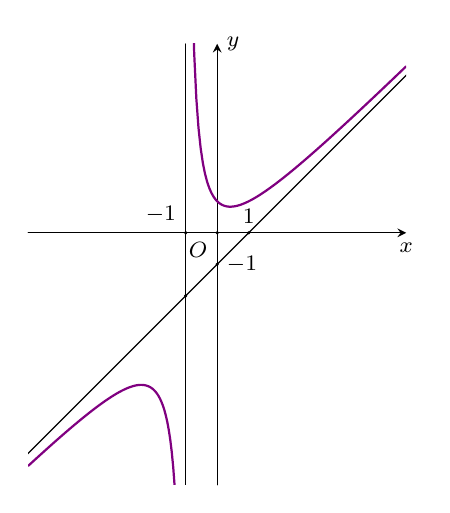
\begin{tikzpicture}[scale=.4, font=\footnotesize, line join=round, line cap=round, >=stealth]
			\draw[->] (-6,0)--(0,0) node[below left]{$O$}--(6,0) node[below]{$x$};
			\draw[->] (0,-8) --(0,6) node[right]{$y$};
			\clip (-6,-8) rectangle (6,6);
			\draw[violet] [domain=-0.8:6, samples=100,thick] %
			plot (\x, {\x-1+ (2)/((\x)+1)});
			\draw[violet] [domain=-6:-1.3, samples=100,thick] %
			plot (\x, {\x-1+ (2)/((\x)+1)});
			\draw[fill] (0,0) circle (1pt) (-1,0) circle (1pt) (-1,-2) circle (1pt) (1,0) circle (1pt)node[above] {$1$} (0,-1) circle (1pt)node[right] {$-1$};
			\draw[domain=-8:7, samples=100] %
			plot (\x, {\x-1});
			\draw (-1,-8)--(-1,0)node[above left] {$-1$}--(-1,6);
	\end{tikzpicture}}
\end{ex}

\begin{ex}
	\immini{Cho đồ thị của hàm số $y=f(x)=\dfrac{2 x^2}{x^2-1}$. Xét tính đúng sai của các khẳng định sau:
	\choiceTF
	{Đồ thị hàm số có 3 điểm cực trị}
	{$\lim \limits_{x \rightarrow-\infty} f(x)=2$ ; $\lim \limits_{x \rightarrow 1^{-}} f(x)=-\infty$}
	{Đồ thị hàm số có 3 đường tiệm cận đứng $x=-1$, $x=0$, $x=1$} 
	{Đồ thị hàm số có hai đường tiệm cận ngang $y=2$ và $y=0$} 
	}{
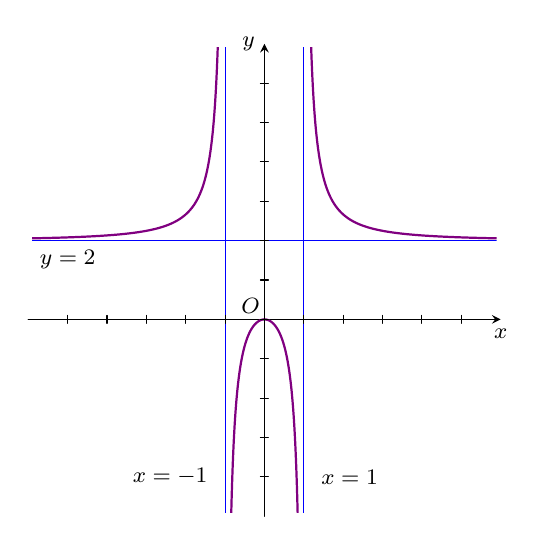
\begin{tikzpicture}[scale=.5,>=stealth, font=\footnotesize, line join=round, line cap=round]
	\def\xmin{-6} \def\xmax{6}
	\def\ymin{-5} \def\ymax{7}
	%\draw[color=gray!50,dashed] (\xmin,\ymin) grid (\xmax,\ymax);
	\draw[->] (\xmin,0)--(\xmax,0) node [below]{$x$};
	\draw[->] (0,\ymin)--(0,\ymax) node [left]{$y$};
	\fill (0,0) circle (1pt) node[shift={(135:2.5mm)}]{$O$};
	\clip (\xmin+0.1,\ymin+0.1) rectangle (\xmax-0.1,\ymax-0.1);
	\draw[thick,smooth,violet,samples=300,domain=(\xmin:-1.01)] plot(\x,{(2*(\x)^2)/((\x)^2-1)});		
	\draw[thick,smooth,violet,samples=300,domain=(-0.9:0.9)] plot(\x,{(2*(\x)^2)/((\x)^2-1)});
	\draw[thick,smooth,violet,samples=300,domain=(1.1:\xmax)] plot(\x,{(2*(\x)^2)/((\x)^2-1)});
	\draw[blue] (\xmin,2)--(\xmax,2);	
	\draw[blue] (-1,\ymin)--(-1,\ymax);	
	\draw[blue] (1,\ymin)--(1,\ymax);		
	\foreach \x in {\xmin,...,\xmax}
	\draw (\x,-0.1)--(\x,0.1);
	\foreach \y in {\ymin,...,\ymax}
	\draw (-0.1,\y)--(0.1,\y);
	\node at (-5,2)[below]{$y=2$};
	\node at (-1.2,-4)[left]{$x=-1$};
	\node at (1.2,-4)[right]{$x=1$};
	%\node at (-1,0)[shift={(-135:2.5mm)}]{$-1$};
	%\node at (.5,0)[shift={(-75:2.5mm)}]{$\dfrac{1}{2}$};
	%\node at (0,-1)[left]{$-1$};
	%\node at (0,2)[shift={(135:2.5mm)}]{$2$};		
\end{tikzpicture}}
	\loigiai{
	\begin{enumerate}[a)]
		\item Đồ thị hàm số có một điểm cực trị $(0;0)$.
		\item Theo hình vẽ thì $\lim \limits_{x \rightarrow-\infty} f(x)=2$; $\lim \limits_{x \rightarrow 1^{-}} f(x)=-\infty$.
		\item Đồ thị hàm số có 2 đường tiệm cận đứng $x= \pm 1$.
		\item Đồ thị hàm số có 1 đường tiệm cận ngang $y= 2$.
\end{enumerate}}
\end{ex}

\Closesolutionfile{ans}
\begin{dang}{Bài toán về đường tiệm cận có chứa tham số}
\end{dang}
\boxmini{BÀI TẬP TỰ LUẬN}
\begin{vd}%[2D1Y4-2]
	Tìm tham số $m$ để đồ thị hàm số 
	\begin{tasks}
		\task $y=\dfrac{3x-1}{x-m}$ có đường tiệm cận đứng là $x=5$.
		\task $y=\dfrac{(m+1)x-5m}{2x-m}$ có tiệm cận ngang là đường thẳng $y=1$.
	\end{tasks}
	\loigiai{
		\begin{enumerate}[a)]
			\item Điều kiện để đồ thị hàm số có tiệm cận đứng là $-3m+1\neq 0\Leftrightarrow m\neq \dfrac{1}{3}$.\\
			Đồ thị hàm số có tiệm cận đứng $x=m$.\\
			Theo đề bài ta có $m=5$ (thoả mãn).
			\item Điều kiện để đồ thị hàm số có tiệm cận ngang là $-m(m+1)+10m\neq 0$.\\
			Tiệm cận ngang là $y=\dfrac{a}{c}=\dfrac{m+1}{2}.$\\
			Theo đề bài ta có $\dfrac{m+1}{2}=1\Leftrightarrow m+1=2\Leftrightarrow m=1$ (thoả mãn).
		\end{enumerate}
	}
\end{vd}

\begin{vd}%[2D1K4-2]
	Tìm $m$ để đồ thị hàm số 
	\begin{tasks}
		\task $y=\dfrac{x-2}{x^2-mx+1}$ có hai đường tiệm cận đứng.
		\task $y=\dfrac{2x^2-3x+m}{x-m}$ có đường tiệm cận xiên.
	\end{tasks}
	\loigiai{
		\begin{enumerate}[a)]
			\item Đồ thị hàm số có hai tiệm cận đứng $\Leftrightarrow$ phương trình $g(x)=x^2-mx+1=0$ có hai nghiệm phân biệt khác $2$.
			$$\Leftrightarrow\heva{&a=1\neq 0 \, (\textrm{LĐ})\\ & \Delta =m^2-4>0\\&g(2)=2^2-2m+1\neq 0} \Leftrightarrow \heva{&\hoac{&m<-2\\&m>2}\\& m\neq \dfrac{5}{2}}.$$
			Vậy $m\in\left(-\infty; -2\right) \cup \left(2; +\infty\right) \setminus \left\{\dfrac{5}{2}\right\}$.
			\item 	Đồ thị hàm số có đường tiệm cận xiên khi và chỉ khi phương trình $g(x)=2x^2-3x+m=0$ không có nghiệm $x=m$. Tức là:
			$$g(m)\neq 0 \Leftrightarrow 2m^2-2m\neq 0 \Leftrightarrow \heva{&m\neq 0\\ &n\neq 1}.$$
			Vậy $m\in\mathbb{R}\setminus\left\{0; 1\right\}$ là các giá trị cần tìm.
		\end{enumerate}
	}	
\end{vd}


\boxmini{BÀI TẬP TRẮC NGHIỆM}
\ind{PHẦN I.} \inden{Câu trắc nghiệm nhiều phương án lựa chọn. Mỗi câu hỏi học sinh chỉ chọn một phương án.}\\
\setcounter{ex}{0}
\Opensolutionfile{ans}[ans/2D1-B3-d3-1]

\begin{ex}
	Tìm tất cả các giá trị của $m$ để đồ thị hàm số $y=\dfrac{mx+2}{x-5}$ có đường tiệm cận ngang đi qua điểm $A(1; 3)$.
	\choice
	{$m=-3$}
	{$m=1$}
	{$m=-1$}
	{\True $m=3$}
	\loigiai{
		Tiệm cận ngang $y=m$ đi qua điểm $A(1; 3)$ nên $m=3$.
	}
\end{ex} 

\begin{ex}
	Tìm tham số thực $m$ để đồ thị hàm số $y=\dfrac{mx+3}{x-m}$ có tiệm cận đứng là đường $x=1$, tiệm cận ngang là đường $y=1$.
	\choice
	{\True $m=1$}
	{$m=2$}
	{$m=-1$}
	{$m=3$}
	\loigiai{
		\begin{itemize}
			\item Điều kiện để đồ thị hàm số có tiệm cận là $-m^2-3\ne 0 \ \forall m$
			\item Phương trình đường tiệm cận đứng là $x=m$ nên có $m=1$
			\item Phương trình đường tiệm cận ngang là $y=m$ nên có $m=1$\\
			Vậy $m=1$.
		\end{itemize}
	}
\end{ex}

\begin{ex}
	Biết rằng hai đường tiệm cận của đồ thị hàm số $y=\dfrac{2x+1}{x-m}$ (với $m$ là tham số) tạo với hai trục tọa độ một hình chữ nhật có diện tích bằng $2$. Giá trị của $m$ là
	\choice
	{$m=\pm 2$}
	{$m=-1$}
	{$m=2$}
	{\True $m=\pm 1$}
	\loigiai{
		Điều kiện $ m\neq -\dfrac{1}{2} $.\\
		Ta có $\lim\limits_{x\to+\infty}\dfrac{2x+1}{x-m}=2$ và $\lim\limits_{x\to-\infty}\dfrac{2x+1}{x-m}=2\Rightarrow y=2$ là tiệm cận ngang của đồ thị hàm số.\\
		\begin{itemize}
			\item Xét $ m>-\dfrac{1}{2} $, ta có $\lim\limits_{x\to m^{+}}\dfrac{2x+1}{x-m}=+\infty$, $\lim\limits_{x\to m^{-}}\dfrac{2x+1}{x-m}=-\infty\Rightarrow x=m$ là tiệm cận đứng của đồ thị hàm số.
			\item Xét $ m<-\dfrac{1}{2} $, ta có $\lim\limits_{x\to m^{+}}\dfrac{2x+1}{x-m}=-\infty$, $\lim\limits_{x\to m^{-}}\dfrac{2x+1}{x-m}=+\infty\Rightarrow x=m$ là tiệm cận đứng của đồ thị hàm số.
		\end{itemize}
		Diện tích hình chữ nhật là $|2m|=2\Rightarrow m=\pm 1$ (thỏa mãn).
	}
\end{ex} 


\begin{ex}
	Tìm giá trị của $m$ để đồ thị hàm số $y=\dfrac{2x^2-5x+m}{x-m}$ có tiệm cận đứng.
	\choice
	{$\hoac{&m=0\\&m=2}$}
	{$m\ne 0$}
	{$m\ne 2$}
	{\True $\heva{&m\ne 0\\&m\ne 2}$}
	\loigiai{
		Ta có $x-m=0\Leftrightarrow x=m$. \\
		Để đồ thị hàm số có tiệm cận đứng thì $2(m)^2-5(m)+m\ne 0\Leftrightarrow 2m^2-4m\ne 0\Leftrightarrow \heva{&m\ne 0\\&m\ne 2}$.
	}
\end{ex} 

\begin{ex}%[2D1Y4-1]
	Tìm tất cả các giá trị thực của tham số $m$ để đồ thị hàm số $y=\dfrac{x-4}{x^2-mx+4}$ có hai đường tiệm cận đứng?
	\choice
	{$m \in \left (-\infty;-4\right] \cup \left [4;+\infty \right )$}
	{$m \ne 5$}
	{\True $m \in \left (-\infty;-4\right) \cup \left (4;+\infty \right ) \setminus \left \{5\right \}$}
	{$m \in \left (-\infty;-4\right) \cup \left (4;+\infty \right )$}
	\loigiai{
		Đồ thị hàm số có hai tiệm cận đứng khi phương trình $x^2-mx+4=0$ có hai nghiệm phân biệt khác $4\Leftrightarrow \heva{&m^2-16>0\\&16-4m+4\ne 0}\Leftrightarrow m \in \left (-\infty;-4\right) \cup \left (4;+\infty \right ) \setminus \left \{5\right \}$ 
	}
\end{ex}

\begin{ex}%[2D1B4-2]
	Cho hàm số $ y = \dfrac{2x^2-3x+m}{x-m} $ có đồ thị $ (C) $. Tìm tất cả các giá trị của tham số $ m $ để $ (C) $ không có tiệm cận đứng.
	\choice
	{\True $ m = 0 $ hoặc $ m = 1 $}
	{$ m = 2 $}
	{$ m = 1 $}
	{$ m = 0 $}
	\loigiai{
		Đồ thị $ (C) $ không có tiệm cận đứng khi $ m $ là nghiệm của $ 2x^2-3x+m $
		\begin{align*}
			\Leftrightarrow 2m^2 - 3m + m = 0 \Leftrightarrow \hoac{& m = 0 \\& m = 1.}
		\end{align*}
	}
\end{ex}

\begin{ex}
	Tìm tất cả các giá trị của tham số thực $m$ để đồ thị hàm số $y=\dfrac{x-2}{x^2-mx+1}$ có đúng $3$ đường tiệm cận.
	\choice
	{\True $\left[\begin{aligned}
			&\left\{\begin{aligned}
				&m>2 \\
				&m\ne \dfrac{5}{2}
			\end{aligned}\right. \\
			&m<-2
		\end{aligned}\right. $}
	{$\left[\begin{aligned}
			&m>2 \\
			&\left\{\begin{aligned}
				&m<-2 \\
				&m\ne -\dfrac{5}{2}
			\end{aligned}\right.
		\end{aligned}\right. $}
	{$\left[\begin{aligned}
			&m>2 \\
			&m<-2
		\end{aligned}\right. $}
	{$-2<m<2$}
	\loigiai{
		ĐKXĐ : $x^2-mx+1\ne 0$ \\
		Ta có $\displaystyle\lim \limits_{x\to \pm \infty}y=\displaystyle\lim \limits_{x\to \pm \infty}\dfrac{x-2}{x^2-mx+1}=0$ $ \Rightarrow y=0$ là tiệm cận ngang. \\
		Do đó đồ thị hàm số $y=\dfrac{x-2}{x^2-mx+1}$ có đúng $3$ đường tiệm cận khi và chỉ khi phương trình $x^2-mx+1=0$ có hai nghiệm phân biệt khác $2$. \\
		$ \Leftrightarrow \left\{\begin{aligned}
			& \Delta =m^2-4>0 \\
			&2^2-2m+1\ne 0
		\end{aligned}\right. \Leftrightarrow \left\{\begin{aligned}
			&\left[\begin{aligned}
				&m>2 \\
				&m<-2
			\end{aligned}\right. \\
			&m\ne \dfrac{5}{2}
		\end{aligned}\right. $. }
\end{ex} 

\begin{ex}
	Cho hàm số $y=\dfrac{ax+1}{bx-2}$, xác định $a$ và $b$ để đồ thị của hàm số trên nhận đường thẳng $x=1$ làm tiệm cận đứng và đường thẳng $y=\dfrac{1}{2}$ làm tiệm cận ngang.
	\choice
	{$ \heva{&a=-1\\&b=-2} $}
	{\True $ \heva{&a=1\\&b=2} $}
	{$ \heva{&a=2\\&b=2} $}
	{$ \heva{&a=2\\&b=-2} $}
	\loigiai{Yêu cầu bài toán $\Leftrightarrow\heva{&\dfrac{a}{b}=\dfrac{1}{2}\\&\dfrac{2}{b}=1}\Leftrightarrow\heva{&b=2\\&a=1}$.}
\end{ex} 


\begin{ex}%[2D1Y4-1]
	Cho hàm số $y=\dfrac{mx+1}{x+3n+1}$. Đồ thị hàm số nhận trục hoành và trục tung làm tiệm cận ngang và tiệm cận đứng. Tính $m+n$.
	\choice
	{\True $m+n=-\dfrac{1}{3}$}
	{$m+n=\dfrac{1}{3}$}
	{$m+n=\dfrac{2}{3}$}
	{$m+n=0$}
	\loigiai{
		\begin{itemize}
			\item Điều kiện để đồ thị hàm số có tiệm cận là $m\left (3n+1\right )\ne 0$
			\item Phương trình đường tiệm cận đứng là $x=-3n-1$ nên có $n=-\dfrac{1}{3}$
			\item Phương trình đường tiệm cận ngang là $y=m$ nên có $m=0$\\
			Vậy $m+n=-\dfrac{1}{3}$.
		\end{itemize}
	}
\end{ex}

\begin{ex}%[2D1K4-2]
	Đồ thị hàm số $y=\dfrac{(4a-b)x^2+ax+1}{x^2+ax+b-12}$ nhận trục hoành và trục tung làm hai tiệm cận. Tính giá trị của $a+b$.
	\choice
	{$a+b=10$}
	{$a+b=12$}
	{$a+b=18$}
	{\True $a+b=15$}
	\loigiai{
		Tiệm cận đứng $x=0 \Rightarrow 0^2+a.0+b-12=0\Leftrightarrow b=12.$\\
		Tiệm cận ngang $y=0 \Rightarrow 4a-b=0\Leftrightarrow 4a-12=0 \Leftrightarrow a=3.$\\
		\textbf{Kết luận:} $a+b=15.$
	}
\end{ex}

\Closesolutionfile{ans}

\ind{PHẦN II.} \inden{Câu trắc nghiệm đúng sai. Trong mỗi ý a), b), c), d) ở mỗi câu, học sinh chọn đúng hoặc sai.}\\
\Opensolutionfile{ans}[ans/2D1-B3-d3-2]
\begin{ex}%[2D1B4-2]
	Cho hàm số $y=\dfrac{mx^2+6x-2}{x+2}$, với $m$ là tham số.
	\choiceTF
	{\True Tập xác định của hàm số là $\mathbb{R}\backslash\{-2\}$}
	{Đồ thị hàm số có tiệm cận ngang khi $m>0$}
	{Đồ thị hàm số có tiệm cận đứng khi $m\ne 0$}
	{\True Tập hợp tất cả giá trị của $m$ đề đồ thị có hai đường tiệm cận là $\mathbb{R}\setminus\left\{\dfrac{7}{2}\right\}$}
	\loigiai
	{
		\begin{enumerate}[a)]
			\item Điều kiện $x+2 \ne 0 \Leftrightarrow x \ne -2$. Vậy Tập xác định là $\mathbb{R}\backslash\{-2\}$
			\item Đồ thị hàm số có tiệm cận ngang khi hệ số của $x^2$ trên tử số phải bằng 0. Suy ra $m=0$.
			\item Đồ thị hàm số có tiệm cận đứng khi $x=-2$ không là nghiệm của tam thức $g(x)=mx^2+6x-2$. Suy ra
			$$g(-2)\ne 0 \Leftrightarrow m \ne \dfrac{7}{2}$$
			\item Đồ thị hàm số chắc chắn có 1 tiệm cận xiên (hoặc ngang). Suy ra, để đồ thị có hai đường tiệm cận thì nó phải có 1 tiệm cận đứng. Điều này tương đương với $m \ne \dfrac{7}{2}$.
		\end{enumerate}
	}
\end{ex}

\Closesolutionfile{ans}
